\documentclass[11pt, letterpaper]{article}
\usepackage{palatino}
\usepackage{graphicx}
\usepackage{enumitem}
\usepackage[top=1in, left=1in, right=1in, bottom=1in]{geometry}

\begin{document}
\begin{center}
\Large{\textbf{Capstone 2 - College Scorecard Data}}

\large{Kirsten Regier}
\end{center}

\section{Introduction}

\textbf{Main question}: What are the primary factors that have contributed to the closing of 4-year undergraduate colleges and universities in the US in the last decade?

According to the https://www.statista.com/ data 'Number of higher education institutions in the U.S. 1980-2017' data, between 2012 and 2017, the number of higher ed institutions decreased by roughly 400.  It could be useful to have a model that is able to predict colleges and universities that are in danger of closing. 
Colleges and universities could use information about common features of schools that have closed to examine their own operational systems, particularly as they face financial difficulties from the coronavirus, which compound the previously existing demographic trends that challenge college enrollment. Insight into which factors that have contributed most significantly in the closing of other colleges could allow current college administrators to make informed decisions about how to protect the future of their institution.

\section{Approach}
\subsection{The Data}
The data was gathered from the US Department of Education's College Scorecard, which is available from https://collegescorecard.ed.gov/data/. The database contains information about schools participate in the Title IV program and accept or distribute federal financial aid to students. Annual data is available from 1996 to 2013; the current analysis focusses on data from 2010 and beyond.

The database includes information about the institution, its finances, federal financial aid and student debt, completion and retention rates, and student demographics. A subset of 15 features were selected for analysis, and narrowed further based on missing data and preliminary modeling. The target variable was a boolean variable that indicates whether the school is currently operating.

\subsection{EDA}
\subsubsection{Governance structure and Predominant degree offered}
Several of the basic features that distinguish different types of schools are their governance structure and the predominant degree offered by the institution. The distribution of the schools by these variables are shown in Table \ref{tab:ControlDegree}. A majority (60\%) of the schools in the dataset are \textbf{private for-profit} schools, and most of these are primarily certificate granting institutions. There are approximately equal numbers of public schools and private non-profit schools, though they differ in the types of degrees offered. The majority of the \textbf{private non-profit} schools offer bachelor's degrees or higher, while more than half of the \textbf{public} schools offer primarily certificates and associate's degrees.

The other variable of interest in Table \ref{tab:ControlDegree} is whether the schools is currently operating or not in a particular year. The data in Table \ref{tab:ControlDegree} includes all schools coded as \textbf{not} currently operating in the database from 2010 - 2013, while the currently operating schools are taken only from the 2013 data. Given the prominence of private for-profit, primarily certificate granting institutions in the data overall, it is not surprising that the majority of the closed schools  (57\%) are also from this category.

\begin{table}[h]
\begin{center}
\begin{tabular}{ l l |c c|c c|c c|| r r }
 \multicolumn{2}{c}{} & \multicolumn{6}{c}{Governance structure} &  \multicolumn{2}{c}{} \\
 \multicolumn{2}{c}{} & \multicolumn{2}{c}{Public} & \multicolumn{2}{c}{Private nonprofit} & \multicolumn{2}{c}{Private for-profit} &\multicolumn{2}{c}{Total}\\
& Operating & No & Yes & No & Yes & No & Yes & No & Yes \\
\cline{2-10}
&Not classified  &  27  & 75& 35 &89 &  191 & 309 & 253 & 473 \\
&Certificate & 117 & 594 & 147 & 199 & 1577 & 2300 &  1841 & 3093\\
\smash{\rotatebox[origin=c]{90}{Degree}} &Associate & 42 & 780 & 26 & 163 & 257 & 545 & 325 & 1488\\
&Bachelor & 13 & 588 & 94 & 1241 & 134 & 271 & 241 &  2100\\
&Graduate & 1 & 15 & 40 & 236 & 58 & 35 &   99 & 286\\
\cline{2-10}
\cline{2-10}
& Total &200 & 2052 & 342 & 1928 & 2217 & 3460 & 2759 & 7440\\
\end{tabular}
\caption{Distribution of schools by predominant degree awarded, governance structure, and whether they are currently operating.}
\label{tab:ControlDegree}
\end{center}
\end{table}

\subsubsection{Enrollment and Cost}
The boxplots in Figure \ref{fig:Control} show the differences in undergraduate student enrollment (left) and cost (right) by governance structure and whether the schools are currently operating. Currently operating public schools have the highest median enrollment and the lowest cost. Private nonprofit schools have the highest median cost and relatively small enrollment numbers, though there are private non-profit schools with relatively large enrollments. Half of the private for-profit schools have enrollment of less than 200 students, but the four schools with the enrollment over 100,000 students %, which are off the scale of the chart in Fig \ref{fig:Control}, 
are also private for-profit schools. Likewise, while the mean cost of the private for-profit schools is lower than that of private nonprofit schools, the schools with the highest cost are also private for-profit schools.

\begin{figure}[h]
\begin{center}
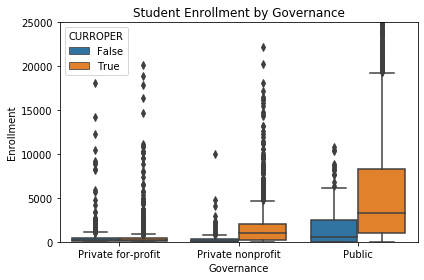
\includegraphics[width=3in]{currentUGDSControlBox.png}
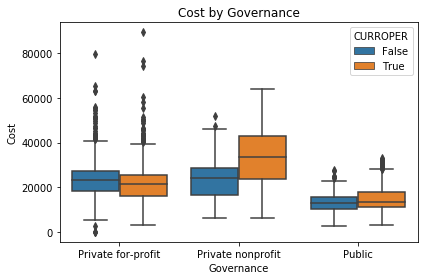
\includegraphics[width=3in]{currentPriceControlBox.png}
\caption{Enrollment (left) and cost (right) of schools by governance structure and whether they are currently operating (CURROPER).  In general, public schools are larger and less expensive than private schools. Private non-profit schools are slightly larger and more expensive than private for-profit schools, though private for-profit schools show more variation in enrollment and cost than private nonprofit schools.}
\label{fig:Control}
\end{center}
\end{figure}

In the swarmplot in Figure \ref{fig:CostDegree}, the cost of currently operating schools is arranged by predominant degree offered and governance structure. This graph highlights that public and private for-profit schools offer mostly certificates and associates degrees, while most private nonprofit schools offer bachelor's degrees (or higher). One reason that private nonprofit schools have the highest median cost could be that they offer higher degrees than most of the public and private for-profit schools. It is also interesting to note that public schools (blue) have lower cost than private for-profit schools (green) regardless of the degree type.

\begin{figure}[h]
\begin{center}
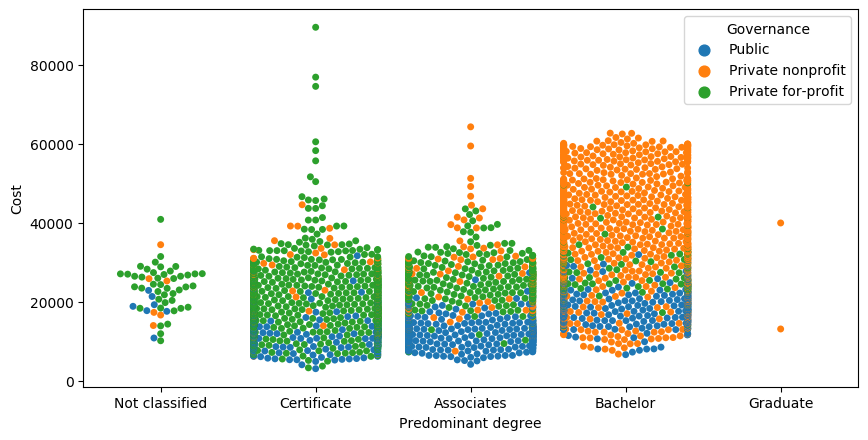
\includegraphics[width=6in]{currentPriceDegreeSwarm.png}
\caption{Cost of currently operating schools by predominant degree offered and governance structure. Private nonprofit schools have higher costs in general, but offer higher degrees than public and private for-profit schools. Public schools generally have lower costs in all degree categories.} 
\label{fig:CostDegree}
\end{center}
\end{figure}

\subsubsection{Other financial metrics}
While student cost and student debt are important financial metrics for students to consider when choosing a school, other financial measures may be informative when considering the financial health of an institution. Several of these features include a school's net tuition revenue per full-time equivalent (FTE) student and instructional expenditure per FTE student. The net tuition revenue per FTE is calculated by subtracting all discounts from tuition revenue, and dividing by the total number of FTE students. The instructional expenditure per FTE is calculated by dividing the instructional expenditure by the number of FTE students. Another potentially important factor could be faculty pay, which is reported in the database as the average monthly faculty salary.

Figure \ref{fig:Correlation} shows heatmaps of the Pearson correlation coefficients between various financial metrics and enrollment for institutions with each type of governance structure. Overall, private for-profit schools show the weakest correlations between most of the financial variables. The most highly correlated features for public schools are cost and debt, while for private nonprofit schools, the highest correlation is between cost and faculty salary, followed closely by cost and tuition revenue.

\begin{figure}[h]
\begin{center}
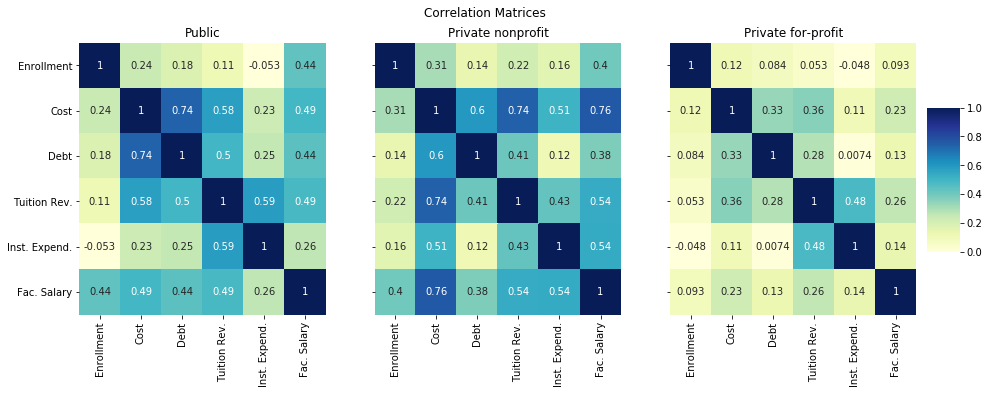
\includegraphics[width=6.5in]{currentFinanceCorrelationHeatmap.png}
\caption{Pearson correlation matrices for various financial metrics by governance type. Darker colors indicate stronger correlations.} 
\label{fig:Correlation}
\end{center}
\end{figure}

\subsubsection{Student characteristics}
While the original plan was to include a variety of information about student demographics, like average SAT/ACT scores, much of this data was either missing or suppressed in the original data. As a result, the only student characteristic that was maintained was the percentage of the student population over the age of 25. As shown in left panel of Figure \ref{fig:Age}, private for-profit schools have the highest percentage of students over age 25, while private nonprofit schools tend to have a slightly lower median percentage than public schools. When divided by predominant degree type (right panel), institutions that offer predominantly bachelor's degree have the youngest populations, and graduate schools have the oldest populations. Interestingly, schools that are not currently operating tend to have higher percentages of students over age 25 than currently operating schools. Since most private nonprofit schools also offer predominantly bachelor's degrees, it is not surprising that these two categories have similar percentages of students over age 25.

\begin{figure}[h]
\begin{center}
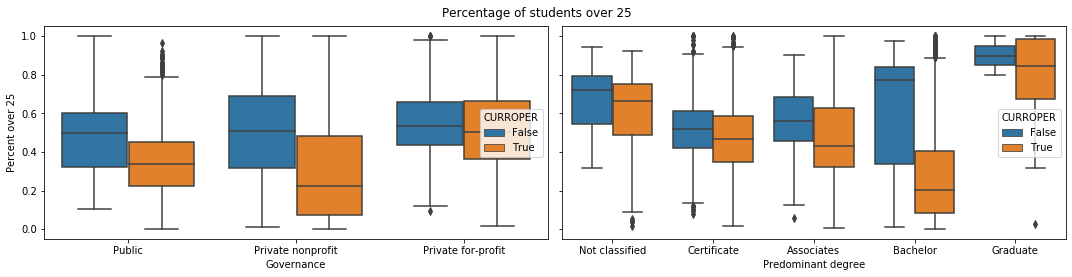
\includegraphics[width=6.5in]{currentOver25Boxes.png}
\caption{Boxplots of the percentage of students over age 25 by school governance structure (left) and predominant degree offered (right).} 
\label{fig:Age}
\end{center}
\end{figure}

\subsection{Data manipulation}
In any given year, there are many fewer schools that are not currently operating than schools that are operating, which led to an unbalanced dataset from the perspective of the target variable (CURROPER). Several methods were explored for balancing the data.

Schools that were not currently operating were extracted from all years (2010 - 2013), while currently operating schools were selected only for the most recent year (2013). This yielded 2759 observations for closed schools and 7440 observations for currently operating schools.

The resampling method that yielded the best balance of overall accuracy and precision \& recall of the closed schools doubled the number of closed schools via random upsampling (with replacement). This resulted in 5518 observations for closed schools, and a total of 12958 observations.

\subsection{Modeling}
The final model included two supervised ML models in series - an initial Decision Tree model that formed the basis for an AdaBoost model. 

 \subsubsection{Decision Tree}
 A grid search was performed to find the optimal hyperparameters (tree depth and node purity method) for the initial decision tree model. The optimal depth was set to 24 and the node purity method was 'entropy'. With the  threshold at 50\% for assigning boolean predictions to the target variable (Currently operating), the overall accuracy for the initial Decision Tree models was 88.9\%, with precision of 83\% and recall of 92\% for the 'Not currently operating' class, as shown in Table \ref{tab:DTConfusion}.
   
\begin{table}[h]
 	\caption{Confusion matrices and Evaluation metrics} 
 	\begin{minipage}{.5\linewidth}
		\caption{Decision Tree Model}
		\centering
		\begin{tabular}{l l | c c r }
\multicolumn{2}{l}{Currently operating} & \multicolumn{2}{c}{Predicted} & Recall \\
& & No & Yes &  \\ 
\cline{2-5}
Actual & No & 1525 &  131 & 0.92 \\
& Yes & 302 &1930 & .86 \\  \hline
Precision&  & .83 & .94 \\ 
Accuracy & & &  & .889 \\
	\end{tabular}
	\label{tab:DTConfusion}
	\end{minipage}%
	\begin{minipage}{.5\linewidth}
	\caption{AdaBoost Model}
	\centering
		\begin{tabular}{l l | c c r }
\multicolumn{2}{l}{Currently operating} & \multicolumn{2}{c}{Predicted} & Recall \\
& & No & Yes &  \\ 
\cline{2-5}
Actual & No & 1536 &  120 & 0.93 \\
& Yes & 171 & 2061 & .92 \\  \hline
Precision&  & .90 & .94 \\ 
Accuracy & & &  & .93 \\
	\end{tabular}
	\label{tab:ABConfusion}
	\end{minipage}
\end{table} 



\subsubsection{AdaBoost Model}
After the initial Decision Tree model was trained, it formed the base for an AdaBoost model. Again, the hyperparameter of the AdaBoost model (n-estimators) was chosen empirically. The AdaBoost algorithm improves model performance by focussing on mis-classified samples and adjusting the model weights to improve their classification. The final AdaBoost model had an overall accuracy of 93\% with a precision of 90\% and recall of 93\% for the 'Not currently operating' class, as shown in Table \ref{tab:ABConfusion}.

\section{Findings}
The weights of different features for the each of the models are given in Figure \ref{fig:Features}. The initial Decision Tree model results suggest that the most important feature in predicting whether a school is currently operating is undergraduate enrollment (UGDS) - the higher the enrollment a school has, the more likely the school is to be currently operating.

While the other features have weights greater than zero, which suggests that they do have predictive power in the model, there are no clear division between features with lesser or greater importance. The other 'top' features include governance (CONTROL), instructional expenditure (INEXPFTE), and percentage of students over age 25 (UG25abv).

The weights of most of the features in the AdaBoost model were null. The only two features that had weights are governance (CONTROL) and completion rate (Complete), and both of these weights are negative, meaning that an increase in these features means it is more likely that the school is not currently operating. Governance (CONTROL) is a categorical feature, meaning that an "increase" in governance is a change in category from public to private nonprofit to private for-profit school. With a negative weight for this feature, it is slightly more likely that private for-profit schools will be not currently operating than public or private nonprofit schools. Given the fact that a majority of the schools in the database are private for-profit schools, it makes sense that a greater percentage of the closed schools are also private for-profit schools, so having this governance structure leads to a greater prediction that the schools will be closed.

\begin{figure}[h]
\begin{center}
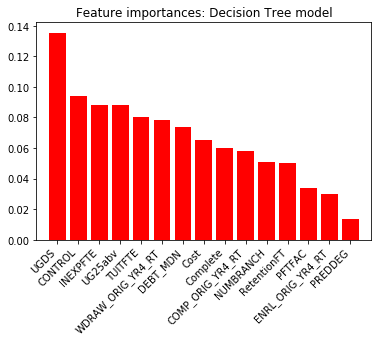
\includegraphics[width=3in]{DTFeatureImportance.png}
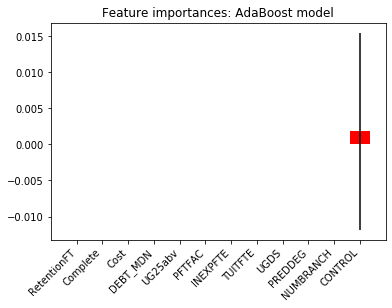
\includegraphics[width=3in]{ABFeatureImportance.png}

\caption{Feature importance levels based on the Decision Tree model (left) and the AdaBoost model (right).} 
\label{fig:Features}
\end{center}
\end{figure}

\subsection{Recommendations}
The Council of Christian Colleges and Universities (CCCU) provides data, support and insight for their more than 180 member colleges and universities. There are several ways that they could use this model to serve their member institutions.

\begin{enumerate}

\item Look at the schools in the test set that were "false negative" results - the ones that the model predicted to be closed, but are actually currently operating. Are there any uniting characteristics, or any special circumstances or institutional changes not accounted for in the model to explain why the schools are still operating, or why the model made the wrong prediction?

For example, the model based on the 2013 test set predicted that 7 private nonprofit bachelor's institutions would be closed. An internet search for those schools showed that they are all currently operating in 2020. It would be interesting to learn more about the individual schools, and see if they were close to closure at any point in the last 7 years, and what changes, if any, they have made recently that would influence their institutional organization or financial situation.

\item Run each of the member schools through the model and examine the predictions. If the model predicts that the school is closed, it could be a warning to school administrators that they need to examine their current operational practices, and make strategic changes.

For example, because I know of several CCCU member institutions with the name 'Bethel', I ran all 15 of the schools whose name starts with 'bethel' through the model. While all of them were correctly predicted, for both currently operating and not currently operating schools, it is likely that some of the 180+ currently operating member institutions would be predicted to be closed.

\item In addition to predicting a boolean value for the schools operating status, the model generates the probability that each school is open (or closed). Even for schools that are predicted to be current operating, it could be insightful to look at the probability associated with the prediction. A school with a 51\% probability of being open could be in more danger of closing than one with a 99\% probability of being open. Examining the probability of individual client schools could provide useful information to the school's administrators.
\end{enumerate}

\section{Future Research}

The most recent data available is from 2013, so there should be five or six years worth of more current data somewhere. It would be interesting to compare the predictions made by the 2013 model to the actual current data, and see how the model and predictions would change if retrained on the more current data. If the goal is of using the model is to help schools weather the financial and economic uncertainty surrounding the coronavirus pandemic, having accurate \textit{current} information about the schools and their financial status would be important.

While the current scorecard data reports on several institutional financial metrics, like tuition revenue, instructional expenditure, and average faculty salary, other financial metrics may provide useful information about the financial status of the institution, that would help make more accurate predictions. Suggested additional data include:
\begin{itemize}
\item the size of the institutional endowment (if any),
\item the amount of institutional debt, or the proportion of institutional debt to the operating budget,
\item the unfunded discount rate - how much financial aid the school provides students apart from federally funded aid
\end{itemize}

Another popular resource for evaluating colleges and universities is the annual US News and World Report rankings. Including information from these rankings, or accessing the data on which the rankings are based, could provide additional metrics and useful features for predicting the closure of institutions.

\end{document}